\documentclass[conference]{IEEEtran}
% Only packages verified to be installed in the local MiKTeX are used
% (booktabs, cite, hyperref, multirow are NOT installed).
% Times (ptm/psnfss) is not installed here; Latin Modern is the cleanest
% fallback. With Times installed, delete the next two lines.
\usepackage[T1]{fontenc}
\usepackage{lmodern}
\usepackage{amsmath,amssymb}
\usepackage{graphicx}
\usepackage{array}
\usepackage{url}
\usepackage{bm}
\usepackage{xcolor}

\graphicspath{{figures/}}
\newcommand{\thetahat}{\hat{\bm\theta}}
\newcommand{\etilde}{\tilde{\bm e}}

\begin{document}

\title{When Does Adaptive Control Need a Universal Function Approximator?\\
A Structure-versus-Capacity Study on a Quadruped Robot}

% NOTE: a line that starts with "[" right after \\ is read as \\[length].
\author{\IEEEauthorblockN{Alp Erem}
\IEEEauthorblockA{KOM 521E Term Project\\
Istanbul Technical University\\
Student No.\ 504251155\\
\texttt{erema19@itu.edu.tr}}}

\maketitle

\begin{abstract}
Classical adaptive control requires the designer to know the
\emph{structure} of the uncertainty; neural-network adaptive control
removes that requirement at the cost of many more parameters. In this
project I ask when that cost is paid back. Starting from two papers---the
adaptive-force-based MPC of Sombolestan and Nguyen~\cite{sombolestan2024}
and the Lyapunov-based deep neural network (Lb-DNN) of Patil
\emph{et~al.}~\cite{patil2022}---I implemented a convex MPC with an
L1-type state predictor on a simulated Unitree~A1 and compared five
adaptive layers with 6 to 390 parameters under matched adaptation gains,
three random seeds and decision rules written before each experiment.
The Lyapunov stability argument of the L1 structure is preserved for
every layer: each update law cancels the cross term of the same
Lyapunov function, the Lyapunov equation is solved explicitly (residual
$3.9\times10^{-17}$), and projection keeps the estimate bounded, giving
uniform ultimate boundedness for a slowly varying disturbance; eight
verification tests, including $\dot V\le0$ for every layer, passed.
Adaptation is necessary: without it the robot cannot finish the combined
course. However, at a well-chosen gain no scenario separated the methods
by success or failure, better estimation did not imply better control,
and almost all of the measurable benefit came from two classical
ingredients: integral action (6 parameters) and knowledge of the gait
phase (12 parameters). A phase-aware classical regressor that contains
both (24 parameters including an error-scaled term that adds nothing at
a well-chosen gain) outperformed the 208-parameter Lb-DNN on a swinging
payload. The classical regressor's
real advantage was tolerance to gain mis-tuning. My answer is that the
approximator becomes necessary when the structure of the disturbance
cannot be written down; for the disturbances studied here, it could.
\end{abstract}

\begin{IEEEkeywords}
adaptive control, L1 adaptive control, model predictive control,
neural networks, legged locomotion, quadruped robots.
\end{IEEEkeywords}

% =====================================================================
\section{Introduction}

A legged robot carrying an unknown payload over uneven ground faces
uncertainty that a nominal model does not capture. Classical adaptive
control handles this well \emph{if} the uncertainty enters the model
through a known regressor: an unknown mass, for example, is just a
number whose place in the equations is known. A foot sinking into mud,
a compliant contact or friction that changes from step to step have no
such clean regressor. Universal function approximators---radial basis
function (RBF) networks~\cite{lewis1996} or deep networks with
Lyapunov-derived update laws~\cite{patil2022}---remove the need to write
the regressor, but they pay for it. Two costs are certain: parameter count
and computation. A third, larger transient overshoot while the many
weights converge, is often expected but has to be measured; in my
payload-step test it did not appear (Section~\ref{sec:res_need},
Table~\ref{tab:quality}), so
the costs that this report actually measures are parameters and
computation (M2's own share is about 15 times that of the classical
regressor).

The research question of this project is therefore:
\emph{when does a universal function approximator become necessary in
adaptive control?} I set out to measure, rather than assume, when its
cost is repaid. Either answer is useful: ``the network wins beyond
condition X'' is a finding, and so is ``classical adaptation is
sufficient and the cost of learning is not repaid''.

My starting point was two papers. Sombolestan and
Nguyen~\cite{sombolestan2024} add an adaptive term to the
single-rigid-body (SRB) MPC of a quadruped and parameterise the
uncertainty with a classical regressor $\bm\alpha\|\bm e\|+\bm\beta$.
Patil \emph{et al.}~\cite{patil2022} derive weight update laws for
\emph{all} layers of a deep network directly from a Lyapunov analysis,
without backpropagation. I implemented both inside the same control
architecture so that the only difference between conditions is the
adaptive layer.

The original proposal of this project was narrower: replace the
uncertainty-estimation block of~\cite{sombolestan2024} with a
Lyapunov-based neural network, keep the stability guarantee, and measure
the performance gain. That experiment is reported in
Sections~\ref{sec:res_need}--\ref{sec:res_est}. When no gain could be
measured, the question widened from ``how much does the network gain?''
to ``when is a network needed at all?'', and the ladder of
Section~\ref{sec:ladder} grew out of that.

\textbf{Contributions.}
\begin{enumerate}
\item A gain-matched, multi-seed comparison of five adaptive layers
(6, 12, 24, 208 and 390 parameters) in one MPC architecture.
\item A ``ladder'' decomposition that isolates what each step of
structure or capacity actually solves.
\item Two hypothesis tests with decision rules written before the
experiments: a speed hypothesis (rejected) and a swinging-payload test
(phase knowledge suffices).
\item A careful re-implementation of~\cite{sombolestan2024}: a sign
error in its kinematic equation, and two implementation details whose
importance I only discovered by measurement.
\end{enumerate}

% =====================================================================
\section{Background}

\subsection{Adaptive-force-based MPC~\cite{sombolestan2024}}
The SRB model of a quadruped is linear in the ground reaction forces
once the yaw rotation is fixed over the horizon~\cite{dicarlo2018}.
Sombolestan and Nguyen augment it with an unknown term and estimate that
term with an L1-style adaptive law~\cite{hovakimyan2010}. Their
parameterisation (Eqs.~(27)/(30) in~\cite{sombolestan2024}) is
\begin{equation}
\thetahat = \hat{\bm\alpha}\,\|\bm e\| + \hat{\bm\beta},
\label{eq:m0}
\end{equation}
where $\bm e=\bm x-\bm x_d$ is the tracking error. The adaptation
direction comes from a separate signal, the state-predictor error
$\etilde$ (Eq.~(41)). This distinction turned out to matter
(Section~\ref{sec:deviations}).

\subsection{Lyapunov-based DNN~\cite{patil2022}}
Patil \emph{et al.} write a $k$-hidden-layer network as
$\Phi(\bm\xi)=V_k^\top\phi_k(\cdots V_1^\top\phi_1(V_0^\top\bm\xi_a))$
and choose the derivative of each weight matrix so that the cross term
in the Lyapunov derivative cancels. For layer $j$,
\begin{equation}
\mathrm{vec}(\dot V_j)=\mathrm{proj}\!\left(\Gamma_j\,
\Big[\Big(\textstyle\prod_{l=j+1}^{k}V_l^\top\phi_l'\Big)
\big(I\otimes\phi_j^\top\big)\Big]^\top \bm s\right),
\label{eq:lbdnn}
\end{equation}
with a Kronecker-product Jacobian (their Eqs.~(7)--(8)). The law is not a
gradient of a loss; there is no data set and no learning-rate schedule.

\subsection{RBF network~\cite{lewis1996}}
The RBF network is linear in its output weights,
$\thetahat=\hat W^\top\bm\phi(\bm\xi)$, with Gaussian bases and the
standard $\sigma$-modification
$\dot{\hat W}=\Gamma\bm\phi\bm s^\top-\sigma\Gamma\hat W$~\cite{ioannou1996}.

% =====================================================================
\section{System and Methods}

\begin{figure*}[t]
\centering
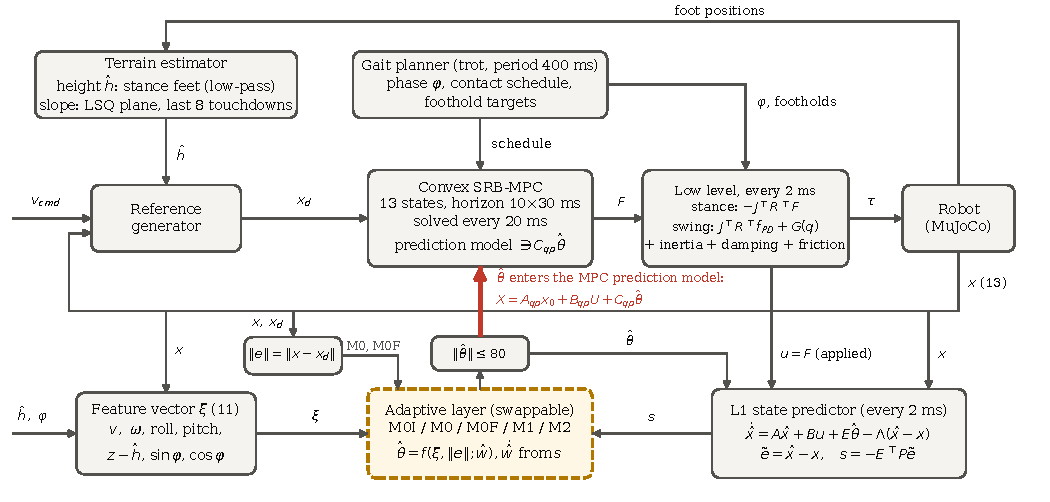
\includegraphics[width=0.95\textwidth]{fig_arch.pdf}\\
{\footnotesize (a)}\\[2pt]
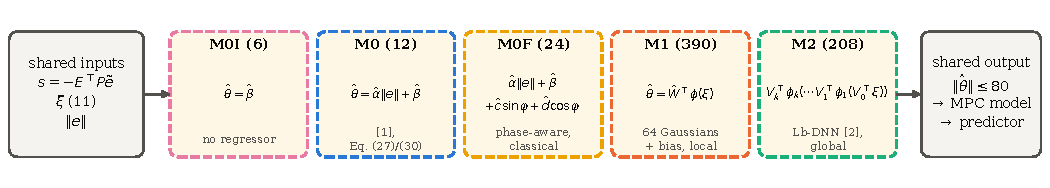
\includegraphics[width=0.95\textwidth]{fig_maps.pdf}\\
{\footnotesize (b)}
\caption{(a) Control architecture. Rates: low level every 2\,ms, MPC
re-solved every 20\,ms (horizon $10\times30$\,ms), trot period 400\,ms;
the state predictor and the adaptive layer run every 2\,ms. The dashed
box is the only element that changes between experimental conditions.
The estimate $\thetahat$ (red) enters the MPC \emph{prediction model}
as an affine term, $X=A_{qp}x_0+B_{qp}U+C_{qp}\thetahat$, held constant
over the horizon; it is not a control signal added to the MPC solution.
This is the same channel as the adaptive MPC of~\cite{sombolestan2024},
where $\bm u_a$ is appended to the state as a constant residual
(Eqs.~(50)--(52)); the difference is that~\cite{sombolestan2024} first
passes the estimate through the low-pass filter $C(s)$, which I measured
and left out (Section~\ref{sec:deviations}). (b) The five layers share
the driving signal $\bm s$, the inputs $\bm\xi$ and $\|\bm e\|$, and the
output bound; only the map from inputs to $\thetahat$ differs.}
\label{fig:arch}
\end{figure*}

\subsection{Robot and baseline controller}
I used the torque-controlled Unitree~A1 model from MuJoCo
Menagerie~\cite{menagerie} in MuJoCo~\cite{todorov2012}.
Fig.~\ref{fig:arch}(a) shows the architecture. The baseline is
a convex SRB-MPC~\cite{dicarlo2018} with a 13-dimensional state, horizon
10, a 30\,ms prediction step, re-solved every 20\,ms; low-level control
runs at 2\,ms. The gait is a trot with a 0.40\,s period. Stance legs
apply $-J^\top R^\top F$; swing legs track a B\'ezier foot trajectory
with a PD force plus gravity, inertia and friction feed-forward.
Swing-leg tracking error was reduced from 24.7 to 4.5\,mm by including
the joint armature, damping and friction of the model. The terrain
height under the robot is the low-pass-filtered mean of the stance feet,
and its slope is a least-squares plane through the last eight
touchdowns.

The baseline MPC has \emph{no integral action}. Against an unknown
constant disturbance it therefore leaves a steady-state error; this
single fact explains most of the baseline behaviour below.

\subsection{Adaptive layer}\label{sec:adaptive}
Following~\cite{sombolestan2024}, the unknown term enters the SRB
dynamics in acceleration units,
$\dot{\bm x}=A\bm x+B\bm u+E\bm\theta$, with
$\bm\theta=[a_x,a_y,a_z,\alpha_x,\alpha_y,\alpha_z]^\top$: a
six-dimensional residual at body level, the linear and angular
acceleration of the trunk that the nominal SRB model does not explain
(payload moments, swing-leg reactions, contact errors). Acceleration
units are a deliberate choice. Expressed as a wrench, the force and
moment channels of $E$ are scaled by $1/m$ and $I^{-1}$, and the
observability matrix $E^\top P(A-\Lambda)^{-1}E$ has a condition number
of 7832, so one scalar gain adapts the force channels about 8000 times
faster than the moment channels. In acceleration units both blocks of
$E$ are identity matrices and the condition number is about 1, so a
single $\gamma$ is meaningful for all six channels. A state predictor
\begin{equation}
\dot{\hat{\bm x}}=A\hat{\bm x}+B\bm u+E\thetahat-\Lambda(\hat{\bm x}-\bm x),
\qquad \etilde=\hat{\bm x}-\bm x
\end{equation}
gives the error dynamics $\dot{\etilde}=(A-\Lambda)\etilde+E\bm\Delta$,
$\bm\Delta=\thetahat-\bm\theta$. With $A_c=A-\Lambda$ Hurwitz
($\Lambda=20I$) and $P\succ0$ solving $A_c^\top P+PA_c=-Q$, the
candidate $V=\etilde^\top P\etilde+\gamma^{-1}\bm\Delta^\top\bm\Delta$
yields
\begin{equation}
\dot V=-\etilde^\top Q\etilde
+2\bm\Delta^\top\!\left(E^\top P\etilde+\gamma^{-1}\dot{\thetahat}\right),
\end{equation}
so the driving signal is $\bm s=-E^\top P\etilde$ and every adaptive
layer distributes $\bm s$ over its own parameters. This is an adaptation
of~\cite{patil2022}, where the weights are driven by the tracking error
$\bm e$ and a robust term $k_s\,\mathrm{sgn}(\bm e)$ is added to the
controller; here all layers share the L1 signal $\bm s$ and no robust
term is used, so that the comparison stays within one architecture
(listed as a deviation in Section~\ref{sec:deviations}).
I solved the Lyapunov
equation explicitly through its Kronecker form (residual
$3.9\times10^{-17}$) rather than calling a library solver. The estimate
$\thetahat$ enters the MPC \emph{prediction model} as an affine term,
not as an additive control signal, and its norm is projected to
$\|\thetahat\|\le80$. Assuming constant $\bm\theta$ gives
$\dot V\le0$; with a slowly varying $\bm\theta$ the result is uniform
ultimate boundedness, which the projection guarantees.

I verified the layer with eight tests (all passed), including a
derived-reference payload test: the slope of $\hat\theta_z$ against
added mass should be $-g/m=-0.788$; I measured $-0.754$ (M2),
$-0.747$ (M0) and $-0.686$ (M1), all with $R^2=1.000$.

\subsection{Five adaptive layers}
Table~\ref{tab:methods} lists the layers and Fig.~\ref{fig:arch}(b)
shows what they share. Every layer receives the same driving signal
$\bm s=-E^\top P\etilde$ and the same inputs (the feature vector
$\bm\xi$ and the tracking-error norm $\|\bm e\|$, each used or ignored
by the map), and every output passes through the same bound
$\|\thetahat\|\le80$ before it reaches the MPC and the predictor. Only
the map from inputs to $\thetahat$, and with it the number of adapted
parameters, differs. M0 is the regressor
of~\cite{sombolestan2024}; M2 is the Lb-DNN of~\cite{patil2022}; M1 is
an RBF network~\cite{lewis1996}. M0I and M0F were added during the
project to isolate the role of structure (Sections~\ref{sec:pendulum}
and~\ref{sec:ladder}). The networks receive an 11-dimensional feature
vector: body linear and angular velocity, roll, pitch, height relative
to the estimated terrain, and $\sin\varphi,\cos\varphi$ of the gait
phase. Position is excluded on purpose, so that the networks cannot
memorise the course. The phase was added because the dominant
disturbance oscillates within the gait cycle: the A1's legs are 62\% of
its mass, so the swing legs produce about $\pm1.4$\,m/s$^2$ of
phase-dependent body acceleration that an SRB model ignores.

\begin{table}[t]
\centering
\caption{Adaptive layers compared (all driven by $\bm s=-E^\top P\etilde$).
Cost: median wall time of one adaptive-layer step and its share of the
2\,ms control period (Python, same machine and run, first 1\,s
discarded, $\approx$4500 calls each). For reference, one MPC solve takes
$\approx$16\,ms in this implementation.}
\label{tab:methods}
\renewcommand{\arraystretch}{1.15}
\setlength{\tabcolsep}{3.5pt}
\begin{tabular}{>{\raggedright}p{0.7cm}>{\raggedright}p{3.15cm}rrr}
\hline
 & form of $\thetahat$ & params & $\mu$s/step & \% of 2\,ms\tabularnewline
\hline
none & no adaptation (baseline MPC) & 0 & -- & --\tabularnewline
M0I & $\hat{\bm\beta}$ (pure integral action) & 6 & 191 & 9.5\tabularnewline
M0 & $\hat{\bm\alpha}\|\bm e\|+\hat{\bm\beta}$ \cite{sombolestan2024} & 12 & 213 & 10.7\tabularnewline
M0F & M0 $+\,\hat{\bm c}\sin\varphi+\hat{\bm d}\cos\varphi$ & 24 & 235 & 11.7\tabularnewline
M1 & RBF, 64 Gaussians + bias, $\sigma=5\times10^{-4}$ \cite{lewis1996} & 390 & 278 & 13.9\tabularnewline
M2 & Lb-DNN, $2\times8$ tanh \cite{patil2022} & 208 & 522 & 26.1\tabularnewline
\hline
\end{tabular}
\end{table}

\subsection{Deviations from the papers}\label{sec:deviations}
\textbf{A sign error.} Eq.~(2) of~\cite{sombolestan2024} writes the
Euler-angle kinematics as $\dot\Theta=R_z\bm\omega$; the correct form is
$\dot\Theta=R_z^\top\bm\omega$. The error is harmless in the paper's
straight-line experiments ($\psi\approx0$, $R_z\approx I$), but I used
the corrected form.

\textbf{Two error signals, not one.} In my first implementation I used
the predictor error $\|\etilde\|$ both as the adaptation direction and
inside the regressor of~\eqref{eq:m0}. Because the update law is itself
driven by $\etilde$, this creates a quadratic positive-feedback loop
$\gamma\|\etilde\|^2$: a larger estimation error enlarges the regressor,
which speeds up adaptation, which enlarges the error. With the paper's
choice---$\|\bm e\|$ (tracking error) in the regressor---M0 at
$\gamma=1000$ went from 0/3 to 3/3 completed runs. The paper's choice
removes the algebraic loop but not a slower one closed through the
plant; Section~\ref{sec:warm} shows it firing under warm start.

\textbf{The low-pass filter $C(s)$ was left out, after measuring it.}
The paper filters the adaptive signal with
$C(s)=\omega_n^2/(s^2+2\zeta\omega_n s+\omega_n^2)$,
$\omega_n=60$\,rad/s, $\zeta=0.7$ (Eqs.~(33)/(45), Table~I). In its MPC
form the filtered signal $\bm u_a=-C(s)\thetahat$ is appended to the
state and held constant over the horizon (Eqs.~(50)--(52)), which is
also how my $\thetahat$ enters the MPC prediction model. In a 54-run
comparison the filter never helped: completion at $\gamma=100/300/1000$
was 8/9, 9/9, 3/9 without and 6/9, 6/9, 3/9 with it. I verified the
filter in isolation (step overshoot 3.4\%, settling 90\,ms), so the
result is not an implementation error. I initially attributed it to the
filter acting on a model term rather than a control signal; on re-reading
Eq.~(50) that explanation does not hold. The clearest remaining
difference is the update rate: their adaptive MPC runs at 300\,Hz
(Section~V-C of~\cite{sombolestan2024}), mine every 20\,ms, so the
$\sim$90\,ms filter lag spans about 27 of their MPC updates but only
4--5 of mine. I did not isolate the cause; the filter is off by
measurement, not by argument.

\textbf{Driving signal of the Lb-DNN.} In~\cite{patil2022} the weights
are driven by the tracking error $\bm e$, and a robust term
$k_s\,\mathrm{sgn}(\bm e)$ is added to the control law. Here M2, like
every other layer, is driven by the L1 predictor signal
$\bm s=-E^\top P\etilde$, and no robust term is used. The layer update
law, Eq.~\eqref{eq:lbdnn}, is unchanged; only its input signal differs,
so that the five layers differ in the map alone. The guarantee is
therefore the L1 one of Section~\ref{sec:adaptive} (uniform ultimate
boundedness),
not the asymptotic tracking result of~\cite{patil2022}, whose proof
relies on the robust term.

\textbf{MPC orientation weight.} With the paper's orientation weight
(0.25, Table~I of~\cite{sombolestan2024}) the A1 fell after 7.8\,s (roll
std 0.43\,rad); I used 5.0 (roll std 0.027\,rad).

% =====================================================================
\section{Experimental Setup}

\begin{figure*}[t]
\centering
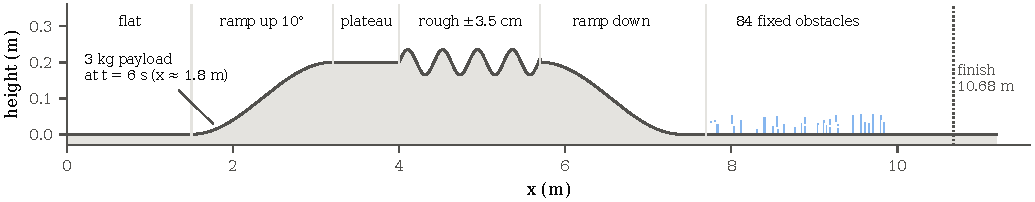
\includegraphics[width=0.92\textwidth]{fig_course.pdf}
\caption{Combined course (schematic height profile; obstacle heights
illustrative). The 3\,kg off-centre payload is attached at $t=6$\,s
without the controller being told. The obstacle field is the hardest
part only in combination with the preceding terrain.}
\label{fig:course}
\end{figure*}

\textbf{Courses.} The main test is the \emph{combined course}
(Fig.~\ref{fig:course}): flat start, a 20\,cm ramp (steepest
$10^\circ$), plateau, rough section ($\pm3.5$\,cm, different left and
right), descent, and 84 fixed obstacles; finish line 10.68\,m, time
limit 60\,s. I also used the terrain part alone (finish 8.0\,m), the
obstacle field alone on flat ground, flat ground (speed test), and a
pendulum scene (Section~\ref{sec:pendulum}). Obstacles are fixed for
measurement: free obstacles are kicked to different places by different
controllers, so the runs would not see the same course.

\textbf{Disturbance.} At $t=6$\,s a 3\,kg payload appears at
$(0.12,0.05,0.06)$\,m in the body frame, producing 3.53\,N\,m of pitch
and 1.47\,N\,m of roll moment. The controller still assumes 12.45\,kg.

\textbf{Gain matching and repetition.} All methods use the same
adaptation gain $\gamma\in\{100,300,1000\}$ (M0 also at 2000 and 3000).
Each cell is run with three seeds (initial weights and RBF centres).

\textbf{Metrics.} A run \emph{completes} if it crosses the finish line;
it \emph{falls} if the trunk drops below 0.12\,m above the local ground
or $|\text{roll}|>1$\,rad; it is \emph{stalled} if it advances less than
5\,cm in 4\,s. The stall detector exists because a collapsed robot was
once reported as ``standing'' for twenty runs. Quality metrics are
averaged over the second (steady) half of each segment: mean $|$pitch$|$,
roll standard deviation and predictor error $\|\etilde\|$.

\textbf{Decision rules.} For every hypothesis test the decision rule was
written into the experiment script \emph{before} running it, and I did
not change it after seeing the results.

\textbf{Reproducibility.} The simulation is deterministic. When I had to
rebuild a scene, I re-ran cells from earlier sweeps and required them to
match to six decimals (they did).

% =====================================================================
\section{Results}

\subsection{Adaptation is necessary}\label{sec:res_need}
Without adaptation the robot stalls on the combined course at 9.01\,m,
independent of gain and seed (Fig.~\ref{fig:baseline}). It does finish
the terrain-only and obstacle-only courses, but with a persistent pitch
error of 0.09\,rad before the payload and 0.12\,rad ($7^\circ$) after it:
the signature of missing integral action. Every adaptive layer reduces
the loaded pitch error 4.5--6.4$\times$ (to 0.019--0.027\,rad,
Table~\ref{tab:quality}). Adaptation does \emph{not} save torque; it lets
the robot finish without saturating it.

\textbf{Transient response.} The payload appearing at $t=6$\,s is a step
disturbance, so I also measured the transient on flat ground (on the
courses the robot is on the ramp or among obstacles at that moment, which
would confound the step). Every adaptive layer limits the first-second
pitch peak to 0.034--0.041\,rad (baseline 0.049) and settles in about
0.9\,s to within 0.004\,rad of its pre-load pitch; the baseline settles
in 1.8\,s but to an offset of 0.029\,rad that never disappears
(Table~\ref{tab:quality}, right). The transient differences between
layers are small: M2 has the lowest peak (0.034) and the fastest mean
settling, but its settling time varies from 0.27 to 0.79\,s between
seeds, while the other layers vary by less than 0.03\,s.

\begin{figure}[t]
\centering
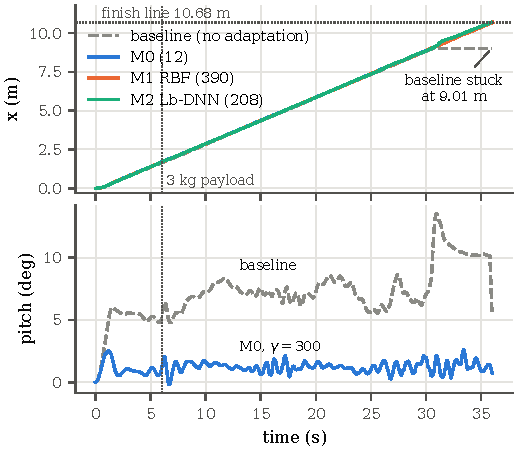
\includegraphics[width=\columnwidth]{fig_baseline.pdf}
\caption{Combined course, $\gamma=300$, seed 0. Top: all adaptive layers
finish; the baseline stalls at 9.01\,m (same in all seeds). Bottom:
pitch, averaged over one gait period; the baseline's offset grows when
the payload appears.}
\label{fig:baseline}
\end{figure}

\subsection{Everyone has a gain window; the classical one is widest}\label{sec:window}
Fig.~\ref{fig:window} shows completion on the combined course.
At $\gamma=300$ every method finishes 3/3. Differences in
success appear only at mis-tuned gains: at $\gamma=1000$ M0 finishes 3/3
while M1, M2, M0F and M0I finish 0/3 (Figs.~\ref{fig:window}
and~\ref{fig:window_xt}); the mis-tuned networks stall at 5.24\,m (M1)
and 5.27\,m (M2), about 3.7\,m short of where the baseline \emph{without}
adaptation stalls (9.01\,m). M0 is
not immune---it fails at $\gamma=2000$ and 3000 (0/3, already on the
ramp)---but its window spans at least a decade (100--1000), wider than
any other layer's.

The $\gamma=1000$ cell of M0 also sits close to that edge. While
recording videos I came across a run of this cell (seed 0) that stalled
at 9.45\,m instead of finishing at 10.68\,m. The only difference was
that the viewer was open, and the passive viewer was then working on the
simulation's own data, which changed the constraint solver's work
buffers. The two runs agree to four decimals in every statistic of the
first six seconds but differ at the bit level from the start. Since then
the viewer draws from a copy, and the run finishes bit-identically to
the headless one. The baseline, M0I at $\gamma=300$ and M2 at
$\gamma=1000$ reproduced their recorded outcomes with the viewer open
even before this fix. That a perturbation small enough to leave the first six
seconds' statistics unchanged to four decimals nonetheless flips this
cell is a single, incidental observation, not an experiment, but it is
consistent with the upper edge lying between 1000 and 2000. All
measurements in this report were run without a viewer.

\begin{figure}[t]
\centering
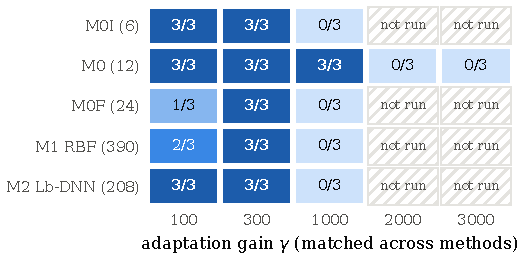
\includegraphics[width=\columnwidth]{fig_window.pdf}
\caption{Completed runs out of three seeds on the combined course, per
method and gain. Darker is better.}
\label{fig:window}
\end{figure}

\begin{figure}[t]
\centering
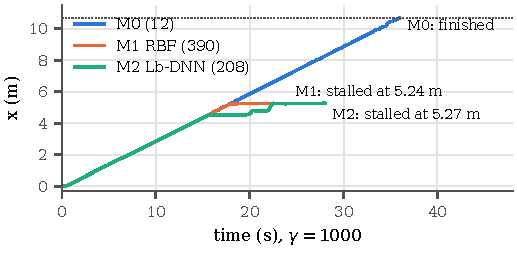
\includegraphics[width=\columnwidth]{fig_window_xt.pdf}
\caption{Combined course at $\gamma=1000$, seed 0: M0 finishes, M1 and
M2 stall in the rough section (5.24 and 5.27\,m). This is a difference in tolerance to
mis-tuning, not in control quality: at $\gamma=300$ all three finish.}
\label{fig:window_xt}
\end{figure}

I first explained the narrower windows by \emph{regressor energy}: the
same $\gamma$ produces a faster total adaptation when
$\|\bm\phi\|^2$ is larger. M0F has about twice M0's regressor energy
($\sin^2+\cos^2=1$ adds one constant channel) and its upper edge is
roughly a factor two lower, which fits. M0I, however, has
\emph{smaller} regressor energy than M0 yet a \emph{narrower} window.
Regressor energy therefore does not explain the window by itself, and I
leave its mechanism open.

\subsection{Better estimation is not better control}\label{sec:res_est}
Table~\ref{tab:quality} reports three-seed means on the two separate
courses at $\gamma=300$, where all methods complete. The pitch ranking
M0 $\le$ M1 $\le$ M2 holds on both courses. The estimation ranking is
decoupled from it: on the obstacle course M1 is the best estimator in
all three seeds but M0 has lower pitch, and M0F is the \emph{worst}
estimator (0.354) yet has the \emph{best} pitch (0.0204). On the terrain
course M2 is the best estimator in two of three seeds while being the
worst in pitch.

\begin{table*}[t]
\centering
\caption{Control quality at $\gamma=300$, mean of 3 seeds (all runs
complete). Left: steady half of the loaded segment; $|\theta_p|$ mean
pitch (rad), $\|\etilde\|$ predictor error. Right: response to the
payload step at $t=6$\,s on flat ground; peak $|\Delta\theta_p|$ in
$[6,7]$\,s relative to the pre-load mean (rad); settling time of the
0.4\,s (one gait period) moving average into $\pm0.01$\,rad of its final
value (band $\ge3\times$ the steady-state fluctuation in every run);
steady offset = final minus pre-load pitch (rad). M0I was added after
the obstacle-course sweep and was not run there (--).}
\label{tab:quality}
\renewcommand{\arraystretch}{1.12}
\setlength{\tabcolsep}{5pt}
\begin{tabular}{lcccccccc}
\hline
 & \multicolumn{2}{c}{terrain only} & \multicolumn{3}{c}{obstacles only} & \multicolumn{3}{c}{payload step, flat ground}\\
 & $|\theta_p|$ & $\|\etilde\|$ & $|\theta_p|$ & $\|\etilde\|$ & roll std & peak $|\Delta\theta_p|$ & settling (s) & steady offset\\
\hline
none & 0.1219 & -- & 0.1216 & -- & 0.0176 & 0.049 & 1.82 & +0.029\\
M0I & 0.0200 & 0.193 & -- & -- & -- & 0.041 & 0.92 & +0.004\\
M0 & 0.0200 & 0.197 & 0.0219 & 0.270 & 0.0167 & 0.039 & 0.89 & +0.003\\
M0F & \textbf{0.0190} & \textbf{0.174} & \textbf{0.0204} & 0.354 & 0.0246 & 0.035 & 0.90 & +0.004\\
M1 & 0.0231 & 0.188 & 0.0225 & \textbf{0.242} & \textbf{0.0158} & 0.040 & 0.90 & +0.004\\
M2 & 0.0253 & 0.204 & 0.0270 & 0.281 & 0.0181 & \textbf{0.034} & 0.58 (0.27--0.79) & +0.004\\
\hline
\end{tabular}
\end{table*}

\subsection{Swinging payload: phase knowledge suffices}\label{sec:pendulum}
To create a disturbance that M0 cannot represent, I hung the 3\,kg
payload on a 4\,cm pendulum (hinge in the roll plane). The length was
chosen \emph{with the baseline only}, before looking at any adaptive
method: at 4\,cm the pendulum resonates with the trot
($g/(2\pi\cdot2.5\,\text{Hz})^2=3.98$\,cm) and swings at 2.50\,Hz with
$10.8^\circ$ standard deviation and near-zero mean
(Fig.~\ref{fig:pendulum_trace}a). Its constant part is solved by
$\hat{\bm\beta}$; its oscillating part has zero mean and is locked to
the gait phase, which M0's regressor does not contain. As a control arm,
the same 3\,kg was welded at the pendulum's rest position (same static
moment), so the difference between the two arms is the oscillation
alone. The modelling detail matters: the hinge is the trunk's
\emph{last} child, so the leg joints keep their state indices, and the
default joint damping of the model (which would lock a pendulum this
light) is overridden.

Pre-registered rule: a layer $M_k$ beats M0 if (a) its predictor error
in the pendulum arm is lower than M0's in at least 8/9 matched cells,
(b) this advantage is larger in the pendulum arm than in the rigid arm
in at least 8/9 cells, and (c) its median roll std is not more than 10\%
worse. Criterion (b) is essential: M2 is already a good estimator on
flat ground, and that advantage must not be credited to the oscillation.

\begin{figure}[t]
\centering
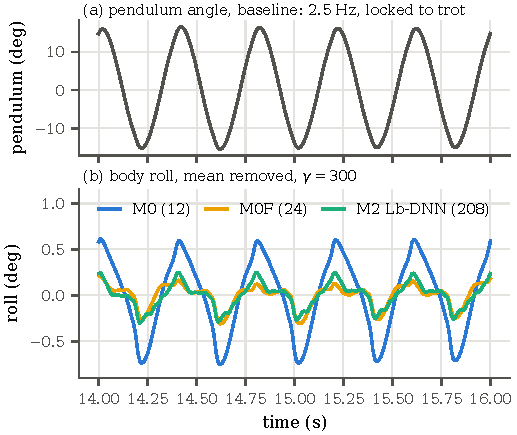
\includegraphics[width=\columnwidth]{fig_pendulum_trace.pdf}
\caption{(a) The 4\,cm pendulum locks to the 2.5\,Hz trot. (b) Body roll
at $\gamma=300$, seed 0: M0F and M2 suppress the phase-locked roll; M0
does not.}
\label{fig:pendulum_trace}
\end{figure}

\begin{figure}[t]
\centering
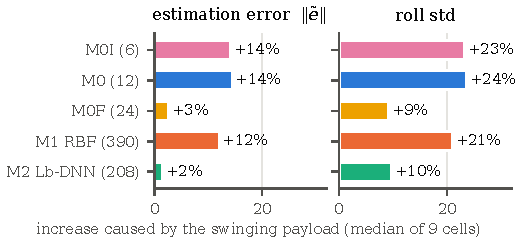
\includegraphics[width=\columnwidth]{fig_pendulum_cost.pdf}
\caption{Cost of the swinging payload: pendulum arm relative to the
rigid arm, same cell, median over 3 gains $\times$ 3 seeds.}
\label{fig:pendulum_cost}
\end{figure}

\textbf{Result.} M2 passed (8/9, 8/9, $-48\%$); M1, although also a
universal approximator, did not ((a) 7/9). The pendulum's extra cost
(Fig.~\ref{fig:pendulum_cost}) is about $+14\%$ estimation error and
$+24\%$ roll for M0 and M1, but only $+2\%$/$+10\%$ for M2. The
estimate of M2 already carries about 5$\times$ more 2.5\,Hz content than
M0's with the \emph{rigid} payload (roll-acceleration channel, 2.98 vs.
0.56 rad/s$^2$), so what puts M2 ahead appears to be that it sees the
gait phase, not its capacity.

I tested this directly with M0F, which is M0 plus the two phase terms:
still a classical, hand-written, linearly parameterised regressor, and
exactly what an engineer who knows the disturbance is gait-periodic
would write. Its rule, also fixed in advance, required passing the M0
test and matching M2 (roll ratio $\le1.10$, pendulum cost within 5
points of M2's). M0F passed every criterion: (a) 9/9, (b) 9/9, roll
$-59\%$ versus M0, roll ratio to M2 0.82, pendulum cost $+3\%$/$+9\%$.
With 24 parameters it matched or beat the 208-parameter Lb-DNN, in both
arms and independently of the seed (Fig.~\ref{fig:pendulum_trace}b).

Two qualifications. All methods, including the baseline, stayed upright;
the differences are in roll quality and small in absolute terms (roll
std $0.45^\circ$ for M0 versus $0.19^\circ$ for M0F at $\gamma=300$).
And at $\gamma=300$ M0 is still about 20\% better than the baseline in
both arms: the pendulum does not cancel M0's benefit, M0 simply cannot
absorb the pendulum's \emph{extra} cost.

\subsection{The ladder: what each step solves}\label{sec:ladder}
Finally I asked whether M0's $\hat{\bm\alpha}\|\bm e\|$ term contributes
anything, using M0I ($\thetahat=\hat{\bm\beta}$, initial $\hat{\bm\beta}$
bit-identical to M0's). At $\gamma\le300$ M0I and M0 are
indistinguishable: identical pitch on the terrain course, roll within
1\% with the pendulum, and both 6/6 on the combined course. The
$\hat{\bm\alpha}\|\bm e\|$ term matters only at high gain, in both
directions: it widens the combined-course window ($\gamma=1000$: M0 3/3,
M0I 0/3) but degrades pendulum roll at the same gain ($\gamma=1000$:
0.0132 vs. 0.0081). Within the
working range, M0 \emph{is} integral action. Table~\ref{tab:ladder}
summarises the ladder.

\begin{table*}[t]
\centering
\caption{The ladder: what each step of structure or capacity adds
(combined course over 9 runs; other columns $\gamma=300$, 3 seeds;
pendulum cost = median over 9 cells)}
\label{tab:ladder}
\renewcommand{\arraystretch}{1.15}
\setlength{\tabcolsep}{4pt}
\begin{tabular}{>{\raggedright}p{1.45cm}>{\raggedright}p{2.5cm}cccc>{\raggedright\arraybackslash}p{5.0cm}}
\hline
step & adds & combined & terrain $|\theta_p|$ & pend. roll & pend. cost & what it solves\\
\hline
baseline (0) & -- & stalls 9.01\,m & 0.1219 & 0.0098 & -- & nothing; MPC lacks integral action\\
M0I (6) & integral action $\hat{\bm\beta}$ & 6/9 & 0.0200 & 0.0079 & +14\% / +23\% & \textbf{constant disturbance}: pitch $6\times$ better, course completed\\
M0 (12) & $+\hat{\bm\alpha}\|\bm e\|$ & \textbf{9/9} & 0.0200 & 0.0079 & +14\% / +24\% & nothing at $\gamma\le300$; \textbf{widens the gain window} upward\\
M0F (24) & $+\hat{\bm c}\sin\varphi+\hat{\bm d}\cos\varphi$ & 4/9 & \textbf{0.0190} & \textbf{0.0034} & \textbf{+3\% / +9\%} & \textbf{phase-locked disturbance}; best pitch; degrades in the obstacle field, narrow window\\
M1 (390) & local universal (RBF) & 5/9 & 0.0231 & 0.0066 & +12\% / +21\% & nothing beyond M0 on the pendulum; best estimator on obstacles\\
M2 (208) & global universal (Lb-DNN) & 6/9 & 0.0253 & 0.0039 & +2\% / +10\% & what M0F solves, with 208 parameters; worst pitch, seed-sensitive\\
\hline
\end{tabular}
\end{table*}

Two steps do real work: integral action for the constant disturbance and
phase knowledge for the phase-locked one. Both are classical
regressors: $\hat{\bm\beta}$ has 6 parameters and the phase terms
$\hat{\bm c},\hat{\bm d}$ have 12, so together they need 18. The
remaining 6 of M0F's 24 belong to $\hat{\bm\alpha}\|\bm e\|$, which adds
nothing at $\gamma\le300$. A caveat: these 18 parameters were never run
on their own, only inside M0F, so ``18 parameters match or beat 208'' is
an inference from the ladder, not a measurement. The universal
approximators did not solve anything measurable beyond these two steps.

\subsection{Warm start: is anything retained?}\label{sec:warm}
Every run above starts from fresh weights. The one advantage a universal
approximator can claim over a classical regressor is that it can
\emph{retain} a state-dependent map, whereas M0 can only retain a
constant. I therefore ran every cell twice on the terrain course
($\gamma=300$, 3 seeds): pass~1 cold, pass~2 starting from the final
weights of pass~1, with the same event schedule (payload at 6\,s). The
predictor, filter and MPC restart in both passes; only the approximator
weights are carried over. Before pass~2 I verified that a loaded weight
file re-saves bit-identically, that with $\gamma=0$ a warm start gives
$\|\thetahat(0)\|=18.6$--$37.1$ instead of ${\approx}0.1$ (so the weights
are really applied), and that a repeated cold pass reproduces pass~1 to
six decimals.

The rule fixed in advance declared $M_k$ ``retaining'' if its
steady-state estimation error in the loaded segment, and in the last
quarter of the run, dropped from pass~1 to pass~2 by more than M0's drop,
in at least two of three seeds. Table~\ref{tab:warm} gives the result.

\begin{table}[t]
\centering
\caption{Warm start on the terrain course, $\gamma=300$, mean of 3 seeds,
pass~1 (cold) $\to$ pass~2 (warm). $\|\etilde\|$ in the steady half of
the loaded segment. Pass~1 is the same run as Table~\ref{tab:quality};
the window here ends one sample (2\,ms) earlier, which moves the fourth
decimal (M2: 0.2034 versus 0.2035).}
\label{tab:warm}
\renewcommand{\arraystretch}{1.12}
\setlength{\tabcolsep}{4pt}
\begin{tabular}{lccc}
\hline
 & completed & loaded $\|\etilde\|$ & loaded $|\theta_p|$\\
\hline
M0I & 3/3 $\to$ 3/3 & 0.193 $\to$ 0.193 & 0.0200 $\to$ 0.0200\\
M0 & 3/3 $\to$ \textbf{0/3} & 0.197 $\to$ \textbf{1.107} & 0.0200 $\to$ 0.0230\\
M0F & 3/3 $\to$ 3/3 & 0.174 $\to$ 0.173 & 0.0190 $\to$ 0.0192\\
M1 & 3/3 $\to$ 3/3 & 0.188 $\to$ 0.188 & 0.0231 $\to$ 0.0231\\
M2 & 3/3 $\to$ \textbf{2/3} & 0.203 $\to$ \textbf{1.330} & 0.0253 $\to$ 0.0372\\
\hline
\end{tabular}
\end{table}

Taken literally, the rule is passed by M1 only. I do not read it that
way. M0, the reference, collapsed under warm start, so ``more than M0's
drop'' became nearly free, and M1's own improvement is 0.0000--0.0002 on
an error of 0.188, about 0.1\%. My rule had no minimum effect size, which
was a flaw. The substantive result is that M0I, M0F and M1 behave the
same warm as cold---whatever they keep is rebuilt within seconds anyway
(M1's $\sigma$-modification also forgets on a ${\approx}7$\,s time
constant)---and that warm start \emph{harms} the two layers with
state-dependent terms. M0's estimate reaches the projection bound (80) on
the rough section and all three seeds fail at ${\approx}5.25$\,m. M0I,
identical except for $\hat{\bm\alpha}\|\bm e\|$, is unaffected, but the
term itself is not the culprit: M0F contains the same term and is also
unaffected. The stored weights show the difference. At the end of
pass~1, $\|\hat{\bm\alpha}\|$ is 6.6--6.7 for M0 but 4.0--4.1 for M0F,
and the pitch-moment component differs most (3.9 versus $-0.1$, all
three seeds). Without a phase regressor, M0 can follow the gait-locked
part of the pitch disturbance only through $\|\bm e\|$, which itself
oscillates with the gait, so that part accumulates in
$\hat{\bm\alpha}$; in M0F the phase coefficients absorb it. Re-running
seed~0 (it reproduces the stored metrics to six decimals) shows warm M0
entering the rough section with $\|\hat{\bm\alpha}\|\approx6.6$ against
$\approx4.3$ when cold. When $\|\bm e\|$ spikes there (to 2.1),
$\hat{\bm\alpha}\|\bm e\|$ reaches 12 in pitch, and because the
$\hat{\bm\alpha}$ update is itself scaled by $\|\bm e\|$ the loop runs
away ($\|\hat{\bm\alpha}\|\to37$). Warm M0F enters with
$\|\hat{\bm\alpha}\|\approx3.0$, smaller than cold M0, and its estimate
never exceeds 32.4.

This is the mechanism of Section~\ref{sec:deviations} seen from the
plant side. There, $\|\etilde\|$ in the regressor closed an
\emph{algebraic} loop $\gamma\|\etilde\|^2$, and the paper's $\|\bm e\|$
broke it. But Eq.~(41) of~\cite{sombolestan2024} still scales the
$\hat{\bm\alpha}$ update by the tracking error,
$\bm y_\alpha=-B^\top P\etilde\,\|\bm e\|$, and the output channel is
$\hat{\bm\alpha}\|\bm e\|$, so during a transient the $\alpha$
contribution again grows like $\|\bm e\|^2$. This time the loop closes
\emph{through the plant}: a large $\thetahat$ degrades control, which
enlarges $\|\bm e\|$, which speeds up $\hat{\bm\alpha}$, which enlarges
$\thetahat$. This explains why the size of $\hat{\bm\alpha}$ alone is
not a threshold. Cold M0 survives $\|\hat{\bm\alpha}\|=9.7$ on flat
ground because $\|\bm e\|$ does not spike there and the loop is never
triggered. The danger is entering a region where $\|\bm e\|$ spikes
while carrying a large $\hat{\bm\alpha}$. M0F is protected because its
phase terms take over the pitch disturbance: $\hat{\bm\alpha}$ stays
small and the loop lacks the initial energy to ignite. To close the
causal question I ran one ablation, with its rule written beforehand:
warm M0 with $\hat{\bm\beta}$ carried over bit-for-bit but
$\hat{\bm\alpha}$ reset to zero. It completed all three seeds with
loaded-segment error 0.198, the same as cold (0.197; full warm start:
0/3, 1.107). The carried $\hat{\bm\alpha}$ is the cause; carrying
$\hat{\bm\beta}$ is harmless but gains nothing. This is the thesis
in another form: correct structure gives each parameter one job, so the
parameters stay well conditioned and transfer safely. M2's estimate saturates at the bound within two
seconds. I suspected my gain-switching rule (it uses $\|\hat V\|$ as a
proxy for the weight error of~\cite{patil2022}, and the warm weights start
above its threshold), but with switching disabled even \emph{cold} M2
stalls at $\gamma=300$ and warm M2 stays saturated, so the damage does not
come from the switching.

What pass~1 leaves behind is therefore not a map but a snapshot of the
last operating point (flat ground, loaded, end of course). For layers
whose output depends on the state, that snapshot is wrong elsewhere and
can push the system to its bounds. The approximator's one distinctive
claim---retaining a mapping---was not observed; warm-starting it was a
risk rather than a benefit.

\textbf{Why nothing is retained, and what would be needed.} The update
$\dot{\thetahat}=-\gamma E^\top P\etilde$ is not a regression: there is
no data set and no loss, and its guarantee is stability, not
identification. Without persistency of excitation (PE) the parameters
are not expected to converge to their true values~\cite{ioannou1996}.
They settle on whatever value cancels the current error. The ``snapshot''
behaviour is therefore the expected outcome, not a defect. The stored
weights show this directly. Comparing seeds is not the right test here:
for the classical layers the seed changes only initial weights of size
$\le0.01$, and the final weights agree to 0--0.6\%, which shows only that
the initial condition is forgotten. For M1 the RBF centres themselves
depend on the seed, and M2 has permutation and sign symmetries, so their
weight vectors (58\% and 143\% apart) are not comparable. The comparable
test is the same history under different parameterisations. The
pitch-moment component of $\hat{\bm\beta}$ agrees within 4\% across
M0I, M0 and M0F (18.3--19.1), but the roll component is $-2.46$, $-1.80$
and $-0.92$. The same physical constant settles on a value that depends
on what the other terms absorb. Likewise M1's bias row, the only part
comparable across seeds, has norm 0.16--0.32, and its roll entry changes
sign between seeds; the constant is spread over the RBFs instead. M1
also cannot retain anything by design, because its $\sigma$-modification
deliberately forgets so that the weights cannot drift. Retention would
need a different addition. Reinforcement learning is the wrong one: it
needs rewards and episodes and gives up the Lyapunov guarantee this
project is built on. The right one is composite or
\emph{concurrent learning}~\cite{chowdhary2010}: a buffer of past
(regressor, uncertainty) pairs adds a data-fit term to the update. Under
a rank condition on the stored data, which is weaker than PE, the
parameters converge and the stability proof is kept. It applies
directly to the linearly parameterised layers (M0F, M1); I leave it to
future work.

% =====================================================================
\section{What I Tried That Did Not Work}\label{sec:tried}

Negative results shaped this project as much as the positive ones. For
each item I give why it was tried, what happened and what I learned.

\textbf{(a) A heavier payload (eliminated without running).} The obvious
way to make the task harder is a heavier payload. I did not run it,
because the outcome follows from the structure: $\hat{\bm\beta}$ is a
pure integrator and removes a constant disturbance of any size, so a
heavier payload would make M0 look \emph{relatively} better. Making the
course harder in general breaks every method at once. Ruling an
experiment out by argument is also a result. It pointed the search
toward disturbances M0 \emph{cannot represent} (the pendulum), rather
than larger ones.

\textbf{(b) The speed axis (null result).} In an early single-seed run
at 0.9\,m/s on the terrain course, M0 fell first and M2 was the best
estimator. This suggested that M0's unbounded regressor $\|\bm e\|$
inflates its effective gain at speed, whereas bounded RBF and tanh
bases do not. I tested this with 4 gains $\times$ 3 seeds at 0.9\,m/s.
On flat ground all methods (and the baseline) stayed up in 12/12 runs.
On the terrain course \emph{all} methods failed 0/12, with falls M0 3,
M1 3, M2 2, and 26 of 28 stalls at the same place (5.4--6.6\,m).
Single runs at 0.6\,m/s also failed for every method. The course defeats
everyone at speed and does not separate the methods; the early ranking
came from a single seed. Lesson: never read a ranking from one seed.

\textbf{(c) The low-pass filter $C(s)$.} The filter is part
of~\cite{sombolestan2024}, so I implemented it, verified it in isolation
and compared it in 54 runs (Section~\ref{sec:deviations}). It never
helped (8/9, 9/9, 3/9 completions without it versus 6/9, 6/9, 3/9 with
it). It remains available as an option. My first explanation was wrong
and had to be retracted, and the likely cause, a 50\,Hz versus 300\,Hz
MPC, was not isolated. Lesson: a design choice can be kept or removed by
measurement even when its mechanism is not yet understood.

\textbf{(d) $\|\etilde\|$ in the regressor.} My first M0 used the
predictor error both as the adaptation direction and as the regressor
magnitude. This closed a quadratic feedback loop $\gamma\|\etilde\|^2$,
and it was the real cause of what I first reported as M0's gain window
(Section~\ref{sec:deviations}). With the paper's $\|\bm e\|$, M0 at
$\gamma=1000$ went from 0/3 to 3/3. Lesson: the two error signals
of~\cite{sombolestan2024} are not cosmetic, and the slower, plant-side
version of the same loop reappeared under warm start
(Section~\ref{sec:warm}).

\textbf{(e) Warm start.} This was tried to test the one advantage left
to the networks, retaining a map (Section~\ref{sec:warm}). Nothing
useful was retained, and the carried weights harmed M0 (0/3) and M2
(error $0.20\to1.33$). Lesson: without persistency of excitation, the
weights are a snapshot of the last operating point, not a map.

\textbf{(f) Eleven silent bugs.} Before the results above were
trustworthy, eleven bugs had to be found. Each made one method look
better or worse than it was, without any error message.
Table~\ref{tab:bugs} lists six of them. They are the methodological
backbone of this report: the first two rules in
Section~\ref{sec:discussion} (suspect the tuning, suspect the metric)
came from them.

\begin{table}[t]
\centering
\caption{Six of the eleven silent bugs found during the project. None
raised an error; each changed a conclusion.}
\label{tab:bugs}
\renewcommand{\arraystretch}{1.12}
\setlength{\tabcolsep}{3pt}
\begin{tabular}{>{\raggedright}p{2.45cm}>{\raggedright}p{3.0cm}>{\raggedright\arraybackslash}p{2.6cm}}
\hline
bug & what it looked like & fix\\
\hline
Height feature absolute, not relative to terrain & ``RBF is fragile'': all 64 bases dead ($\phi\approx10^{-13}$), M1 a constant on 55\% of the course & height relative to the estimated terrain\\
M1 without a bias term & M1 a weak estimator: bases near a steady $\bm\xi\approx0$ stay at $\phi\approx0.08$, none excited & bias added (error 0.67$\to$0.45)\\
M2's switched gain used $\|\hat V\|$, which grows monotonically & M2 locked at an absolute low gain (effectively $\gamma=1$) & threshold $3\times$ initial norm, low gain $\gamma/10$\\
All methods compared at $\gamma=1000$ & ``networks fail'' & matched gain sweep (100--1000)\\
Collapsed robot reported as standing & 20 runs ``successful'' (only sign: $v_x=0$) & stall detector\\
Robot fell off the map edge at $x=12$\,m & ``adaptation costs torque'' & finish line\\
\hline
\end{tabular}
\end{table}

\textbf{(g) What remains open.} Two observations are still unexplained.
First, M0F's lower gain edge: at $\gamma=100$ two of three seeds stall
on the combined course at 9.00\,m, where the baseline stalls. The
regressor-energy argument does not explain this, since M0F at
$\gamma=100$ adapts roughly like M0 at $\gamma=200$, well inside M0's
window. Second, the mechanism of the gain window: regressor energy fits
M0F's upper edge but not M0I's, whose energy is smaller than M0's while
its window is narrower (Section~\ref{sec:window}).

% =====================================================================
\section{Discussion}\label{sec:discussion}

\textbf{Structure versus capacity.} What improved control was structure
that matches the disturbance, not capacity. Structure helps only when
the disturbance actually has it: M0F is the best layer where locomotion
is regular (terrain, pendulum), but in the obstacle field, where the
gait is disrupted and the disturbance is no longer phase-locked, its
phase terms learn the wrong thing (worst estimation 0.354 and worst roll
0.0246 there), and on the combined course its window is narrow (4/9).

\textbf{Gain matching is not neutral.} The same $\gamma$ is not the same
effective adaptation rate across parameterisations. Matching $\gamma$ is
the natural experimental control, but it is itself a cost: a gain tuned
for the classical design does not transfer to a network.

\textbf{Transient cost.} Transient overshoot is commonly listed among
the costs of an approximator. In the payload step test I did not observe
it: no layer overshoots more than the classical ones, and M2 has the
lowest peak. The cost that does appear is variability between seeds
(M2's settling time spans a factor of three), consistent with its
seed-sensitivity elsewhere.

\textbf{Computation.} The adaptive layer costs 9.5--26\% of the 2\,ms
control period in my Python implementation (Table~\ref{tab:methods}).
About 190\,$\mu$s of that is the shared state predictor, which every
layer needs; the approximator itself adds 22\,$\mu$s (M0), 44 (M0F), 87
(M1) and 331\,$\mu$s (M2) on top. The Lb-DNN's own share is therefore
about 15 times that of the classical regressor, for a layer that did not
outperform the 24-parameter M0F. The absolute numbers are specific to
Python (one MPC solve takes $\approx$16\,ms here); the ratios are the
transferable part.

\textbf{Lessons on method.} Three claims I had written during the
project did not survive repetition, and all three had the same cause:
(i) the speed effect came from a single seed; (ii) ``M1 is the best
estimator on all four segments'' held on only two of four with three
seeds; (iii) ``the pendulum cancels M0's benefit'' came from a 9-cell
mean dominated by one high-gain cell. Earlier, eleven silent bugs had
made one method or another look better or worse than it was
(Table~\ref{tab:bugs}). The practical rules I adopted are: suspect your own tuning before declaring a method
worse, suspect your own metric before declaring a run successful, never
read a ranking from one seed, and write the decision rule before the
experiment.

\textbf{Limitations.} Two disturbance types (constant payload, one
pendulum setting), one payload position, a sparse gain grid, and
simulation only. Warm start was tested only as a second pass over the
same course (Section~\ref{sec:warm}); transfer of stored weights to
different conditions was not tested. An 18-parameter layer with only
$\hat{\bm\beta}$ and the phase terms (M0F without
$\hat{\bm\alpha}\|\bm e\|$) was not run; its performance is inferred from
the ladder. Two observations remain unexplained
(Section~\ref{sec:tried}(g)).

% =====================================================================
\section{Conclusion}

Adaptation was necessary: without it the quadruped could not complete
the combined course. Beyond that, better estimation did not mean better
control, and the measurable benefit came from two classical, hand-written
pieces of structure---integral action and gait-phase knowledge, 6 and
12 parameters. Measured inside the 24-parameter M0F, which also carries
an error-scaled term that adds nothing at a well-chosen gain, they
matched or beat a 208-parameter Lyapunov-based DNN on a phase-locked
swinging payload. The classical regressor's
real advantage was its tolerance to gain mis-tuning. Warm-starting the
networks did not show them retaining a useful map; for the layers with
state-dependent terms it was harmful. I found no scenario
in which a universal approximator accomplished a task the classical
design could not.

My answer to the research question is therefore: \emph{a universal
function approximator becomes necessary when the structure of the
disturbance cannot be written down.} For the disturbances studied
here---an unknown payload, gait-induced leg dynamics and a phase-locked
pendulum---it could. The natural next step is a disturbance whose
structure is genuinely hard to write, such as sinking or compliant
ground with a per-foot $\bm\theta$. A second step is concurrent
learning~\cite{chowdhary2010}. Without persistency of excitation none of
the layers identifies its parameters, so none can retain a map; a buffer
of recorded data would give parameter convergence without giving up the
stability guarantee, and only then can the claim that an approximator
retains a map be tested fairly.

% =====================================================================
\section*{Code availability}
The complete source code (controller, the five adaptive layers, course
generation, every sweep script with its pre-registered decision rule and
the figure scripts) is provided as a supplementary archive with this
report, together with the raw sweep outputs. All runs are deterministic
for a given seed; earlier cells were re-run after each code change and
reproduced to six decimals.

% =====================================================================
\begin{thebibliography}{9}

\bibitem{sombolestan2024}
M.~Sombolestan and Q.~Nguyen, ``Adaptive-force-based control of dynamic
legged locomotion over uneven terrain,'' \emph{IEEE Trans. Robot.},
vol.~40, pp.~2462--2477, 2024.

\bibitem{patil2022}
O.~S.~Patil, D.~M.~Le, M.~L.~Greene, and W.~E.~Dixon, ``Lyapunov-derived
control and adaptive update laws for inner and outer layer weights of a
deep neural network,'' \emph{IEEE Control Syst. Lett.}, vol.~6,
pp.~1855--1860, 2022.

\bibitem{lewis1996}
F.~L.~Lewis, A.~Ye\c{s}ildirek, and K.~Liu, ``Multilayer neural-net robot
controller with guaranteed tracking performance,'' \emph{IEEE Trans.
Neural Netw.}, vol.~7, no.~2, pp.~388--399, 1996.

\bibitem{dicarlo2018}
J.~Di~Carlo, P.~M.~Wensing, B.~Katz, G.~Bledt, and S.~Kim, ``Dynamic
locomotion in the MIT Cheetah~3 through convex model-predictive
control,'' in \emph{Proc. IEEE/RSJ IROS}, 2018, pp.~7440--7447.

\bibitem{hovakimyan2010}
N.~Hovakimyan and C.~Cao, \emph{$\mathcal{L}_1$ Adaptive Control
Theory: Guaranteed Robustness with Fast Adaptation}. Philadelphia, PA, USA: SIAM, 2010.

\bibitem{ioannou1996}
P.~A.~Ioannou and J.~Sun, \emph{Robust Adaptive Control}. Upper Saddle
River, NJ, USA: Prentice Hall, 1996.

\bibitem{chowdhary2010}
G.~Chowdhary and E.~Johnson, ``Concurrent learning for convergence in
adaptive control without persistency of excitation,'' in \emph{Proc.\
49th IEEE Conf.\ Decision Control (CDC)}, 2010, pp.~3674--3679.

\bibitem{todorov2012}
E.~Todorov, T.~Erez, and Y.~Tassa, ``MuJoCo: A physics engine for
model-based control,'' in \emph{Proc. IEEE/RSJ IROS}, 2012,
pp.~5026--5033.

\bibitem{menagerie}
K.~Zakka, Y.~Tassa, and MuJoCo Menagerie contributors, ``MuJoCo
Menagerie: A collection of high-quality simulation models for MuJoCo,''
2022. [Online]. Available: \url{https://github.com/google-deepmind/mujoco_menagerie}

\end{thebibliography}

\end{document}
